\begin{pastexam}[label={px:ncku-114-ee-ds-08}]{成大電機所 114 學年度 單選題第 8 題}
（單選；每題 5 分，答錯倒扣 2 分）

Prim algorithm is used to construct a minimum spanning tree $T$ by using the data structure
``set''. They form a set for all nodes in the beginning and gradually merge two nodes until $T$ is
found. Please identify the first edge which form a cycle in $T$ during the procedure and the
number of sets formed at that moment.

\begin{center}
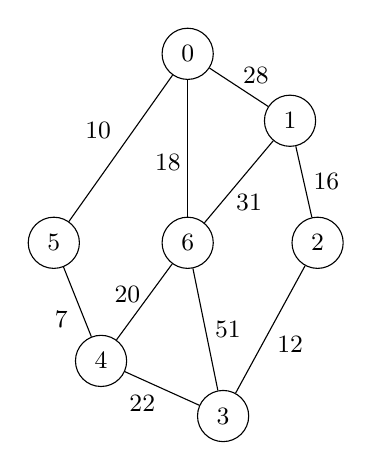
\begin{tikzpicture}[v/.style={draw,circle,minimum size=6.5mm,inner sep=0pt},font=\small]
  \node[v] (0) at (0,0) {0};
  \node[v] (1) at (1.3,-0.85) {1};
  \node[v] (5) at (-1.7,-2.4) {5};
  \node[v] (6) at (0,-2.4) {6};
  \node[v] (2) at (1.65,-2.4) {2};
  \node[v] (4) at (-1.1,-3.9) {4};
  \node[v] (3) at (0.45,-4.6) {3};
  \draw (0) -- node[above right=-2pt] {28} (1);
  \draw (0) -- node[above left] {10} (5);
  \draw (0) -- node[left=-1pt,pos=0.6] {18} (6);
  \draw (1) -- node[below right=-2pt,pos=0.6] {31} (6);
  \draw (1) -- node[right] {16} (2);
  \draw (5) -- node[below left] {7} (4);
  \draw (6) -- node[left,pos=0.4] {20} (4);
  \draw (6) -- node[right] {51} (3);
  \draw (2) -- node[below right=-1pt] {12} (3);
  \draw (4) -- node[below left=-1pt] {22} (3);
\end{tikzpicture}
\end{center}

a) edge (3, 6) and 2 set \quad b) edge (4, 6) and 4 set

c) edge (0, 1) and 3 set \quad d) edge (4, 6) and 3 set

e) None of the above
\end{pastexam}

\begin{pastsoln}
答案是 b) edge (4, 6) and 4 set。

\textbf{題意。} 題目說用 Prim，又說「一開始每個點一個集合、逐步合併」，後者比較像 Kruskal 的寫法。
選項 b)、d) 都是 $(4, 6)$，差在集合個數，兩種讀法算一次就知道出題的意思：
\begin{itemize}
\item 照 Prim（從頂點 $0$ 開始，資結書第~24.3~節）：已在樹上的頂點是一個集合，其他每個頂點各自
一個集合。 每次取「一端在樹上」的邊裡最輕的一條；兩端都已在樹上的邊會成環，丟掉。
\item 照 Kruskal（資結書第~24.2~節）：邊由輕到重看，兩端在同一集合就成環。
\end{itemize}

\textbf{Prim，從 $0$ 開始}：
\begin{center}
\begin{tabular}{llll}
\toprule
步驟 & 取出的最輕候選邊 & 結果 & 集合 \\
\midrule
1 & $(0, 5)$ 10 & 加入 $5$ & $\{0, 5\}, \{1\}, \{2\}, \{3\}, \{4\}, \{6\}$ \\
2 & $(5, 4)$ 7 & 加入 $4$ & $\{0, 4, 5\}, \{1\}, \{2\}, \{3\}, \{6\}$ \\
3 & $(0, 6)$ 18 & 加入 $6$ & $\{0, 4, 5, 6\}, \{1\}, \{2\}, \{3\}$ \\
4 & $(4, 6)$ 20 & \textbf{兩端都在樹上，成環} & 仍是 $4$ 個集合 \\
\bottomrule
\end{tabular}
\end{center}
第 3 步時候選邊有 $(0, 6)$ 18、$(4, 6)$ 20、$(4, 3)$ 22、$(0, 1)$ 28，取 $18$；第 4 步最輕的候選是
$(4, 6)$ 20，但 $4$、$6$ 都已在樹上，它是第一條會成環的邊，這時有 $\{0, 4, 5, 6\}, \{1\}, \{2\},
\{3\}$ 共 $4$ 個集合，就是 b)。 之後依序加入 $(4, 3)$ 22、$(3, 2)$ 12、$(2, 1)$ 16，最小生成樹
總權重 $10 + 7 + 18 + 22 + 12 + 16 = 85$。

\textbf{Kruskal 的話}：$7$ $(4,5)$、$10$ $(0,5)$、$12$ $(2,3)$、$16$ $(1,2)$、$18$ $(0,6)$ 都加入，集合
從 $7$ 個合併到剩 $\{0, 4, 5, 6\}, \{1, 2, 3\}$ 兩個；下一條 $20$ $(4, 6)$ 兩端同集合，成環。 第一條
成環的邊也是 $(4, 6)$，但這時只有 $2$ 個集合，選項裡沒有，要選 e)。

題目寫的是 Prim，照 Prim 算出的 b) 也在選項裡，所以答 b)。 其他選項：a) $(3, 6)$ 51 是最重的邊，
很晚才會被看到；c) $(0, 1)$ 28 在 $(4, 6)$ 之後；d) 集合數不對。
\end{pastsoln}
